\section{Difficulty Levels}
\index{Difficulty levels}
\label{core:difficulty-rating}

While \emph{The Wyrd Engine} uses a simple resolution mechanic, it is important to establish how difficult a given action is. The Game Master determines the \textbf{Difficulty Rating (DR)} based on the complexity of the task, the environment, and any obstacles the characters may face.

\subsection{Passive Opposition}
\index{Passive opposition}
The \textbf{Difficulty Rating (DR)} represents the challenge level of a task. The simplest tasks involve no active opposition—where success or failure is determined solely by the character’s own abilities. This could be deciphering an ancient cipher, scaling a rocky cliff, or crafting a delicate mechanism—situations where the only obstacle is the task itself, rather than an opposing force.

In these cases, the player rolls \textbf{4dF} + their \textbf{Skill Modifier} and applies any relevant \textbf{Trait} or \textbf{Gear bonus} (Gear Traits). If the total meets or exceeds the DR, the action succeeds.

The GM determines the difficulty rating based on two factors: how inherently challenging the task is and how critical it is to the game’s progression. A well-balanced difficulty keeps the players engaged—offering real challenges without creating dead ends. While setbacks can enrich the story, a GM should never impose an insurmountable barrier that halts progress entirely. Instead, every challenge should be an opportunity for clever thinking, teamwork, and dramatic tension.

The following table can guide you in determining the difficulty rating for a task:

\begin{DndTable}[header=Difficulty Levels in \emph{The Wyrd Engine}]{lX}
    \textbf{Difficulty Rating} & \textbf{Example Task}\\
    \hline
    \Trivial & A task so easy that failure is nearly impossible (walking across a stable floor, recalling your own name). \\
    \Simple & A straightforward action requiring minimal effort (identifying a common herb, climbing a ladder). \\
    \Easy & A minor challenge that most people can accomplish without effort (jumping over a puddle, recalling common knowledge). \\
    \Basic & An ordinary action requiring some attention (spotting a misplaced item, balancing on a narrow beam). \\
    \Challenging & A moderate test of skill or effort (spotting a hidden compartment, climbing a wooden fence). \\
    \Difficult & A task requiring training or experience (tracking footprints in the rain, persuading a sceptical guard). \\
    \Formidable & A demanding task that pushes a character’s limits (picking a complex lock under pressure, leaping between rooftops). \\
    \Arduous & A near-impossible feat requiring mastery (detecting a forged document at a glance, sniping a target from extreme range). \\
    \Extreme & A task on the edge of human capability (convincing a lifelong enemy to trust you, performing surgery in total darkness). \\
    \Impossible & A superhuman achievement defying all odds (dodging bullets mid-air, convincing an ancient dragon to surrender). \\
\end{DndTable}

For levels up to \Basic, rolls are usually unnecessary unless dramatic tension is involved. For characters with appropriate skills, \Basic tasks can also be handled without rolls.

We can superimpose the difficulty levels on the 4dF success rate graph to directly visualise how difficult it will be with just dice rolls to reach a given level:

\begin{center}
	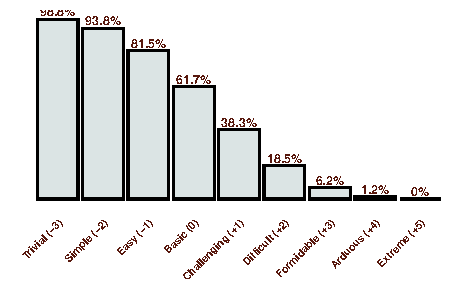
\includegraphics{stats/4dF-DR.pdf}
\end{center}

The graph tells us that even \Trivial tasks can fail if you are unskilled and unlucky enough, and \Challenging tasks will fail a third of the time for someone without the necessary skills.

Adding skills effectively shifts the difficulty levels. When playing the game, we add skill levels to the 4dF rolls, as this is the easiest way to calculate the result, but when setting difficulty levels, it is easier to think in terms of how difficult an unskilled character would find a task, and then shift the difficulty levels down by one for each skill level a character has.

A skill level of \Novice adds one to the 4dF, which effectively shifts the difficulties down by one. If we are adding \textbf{+1} to a roll, the unmodified range of \textbf{-4} to \textbf{+4} for a \Untrained character instead becomes the shifted range of \textbf{-3} to \textbf{+5}, for example. With this switch, the difficulty with which a \Novice character hits a \Challenging level will be the same as if he only had to reach the \Basic level.

\begin{center}
	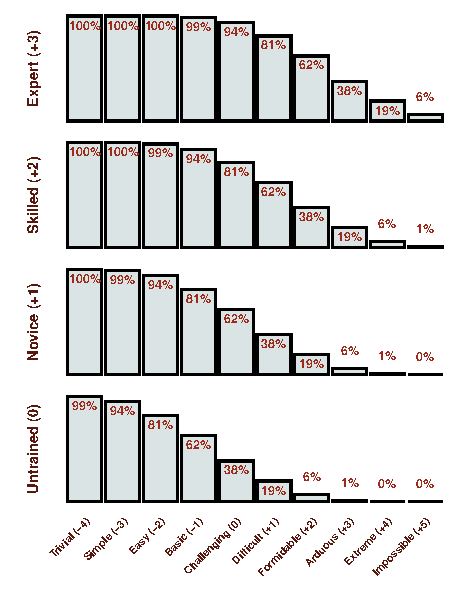
\includegraphics{stats/shifted-DR.pdf}
\end{center}

A \Basic task, which has a 2/3 chance of success for an \Untrained character will be a success one out of twenty for a \Novice and a guaranteed success for an \Expert character. An \Extreme task, which will be impossible for an \Untrained and not much easier for a \Novice, has a one-in-five chance of success for an \Expert. Add in a \textbf{Trait (+2)}---which shifts the range by an additional two points---and an \Expert character will, under the right circumstances, have a one-in-three chance of doing the impossible.

The table below shows the probability of success for the different difficulty levels at different skill levels:

\begin{DndTable}[header=Success probability per skill level]{lrrrr}
    \textbf{Difficulty} & \textbf{0} & \textbf{+1} & \textbf{+2} & \textbf{+3} \\
    \hline
    \Trivial     & 98.8\% & 100.0\% & 100.0\% & 100.0\% \\
    \Simple      & 93.8\% &  98.8\% & 100.0\% & 100.0\% \\
    \Easy        & 81.5\% &  93.8\% &  98.8\% & 100.0\% \\
    \Basic       & 61.7\% &  81.5\% &  93.8\% & 98.8\% \\
    \Challenging & 38.7\% &  61.7\% &  81.5\% & 93.8\% \\
    \Difficult   & 18.5\% &  38.7\% &  61.7\% & 81.5\% \\
    \Formidable  &  6.2\% &  18.5\% &  38.7\% & 61.7\% \\
    \Arduous     &  1.2\% &   6.2\% &  18.5\% & 38.7\% \\
    \Extreme     &  -     &   1.2\% &   6.2\% & 18.5\% \\
    \Impossible  &  -     &   -     &   1.2\% &  6.2\% \\
\end{DndTable}

Players will not need to consult this table during a game---in \emph{The Wyrd Engine} we are not keen on using tables for game mechanics---but it should give a Game Master a rough idea of how to set difficulty levels when planning a game session.


\begin{DndComment}{Game Master Tip}
	When deciding on difficulty levels, you should focus on the narrative aspects of the game rather than realism in difficulty. You want to give the players exciting challenges, but any conflict resolution should have narrative relevance. Don't ask for dice rolls if you can act out a scene instead, and don't ask for dice rolls unless both failure and success will have exciting consequences. It is okay to have automatic wins and automatic losses if the alternative will break the story you are trying to tell, and it is okay to set unrealistically low or high difficulty levels if that is what it takes to tell a good story.
	\end{DndComment}



\subsection{Active Opposition}
\index{Active opposition}
When two characters compete directly but are not in combat (for that, see below), both roll \textbf{4dF + their relevant skill}. The highest result wins.

\begin{itemize}
    \item If one character beats the other by \textbf{1 or 2 points}, they succeed with a minor advantage.
    \item If they beat the other by \textbf{3 or more points}, their success is so impressive that the GM can, at their discretion, provide the winning character with a \textbf{boon}.
\end{itemize}

A \textbf{boon} is a one-use trait invented for the situation at hand. It is only active for the current scene and is lost if not used after the scene ends.

\subsection{Ties and Partial Successes}
\index{Ties}\index{Partial successes}
Not every roll results in a clean success or failure. When a roll \textbf{ties} the Difficulty Rating, or when failure would halt progress entirely, the GM may introduce a \textbf{complication}:

\begin{itemize}
    \item \textbf{Success with a Cost:} The action succeeds, but at a price (e.g., escaping a pursuer but losing an important clue).
    \item \textbf{Mixed Success:} The character achieves part of their goal, but not completely (e.g., unlocking a door but setting off an alarm).
    \item \textbf{A New Complication:} The failure introduces an unexpected twist (e.g., picking a lock only to find guards already inside).
\end{itemize}

\subsection{Interpreting Failure}
\index{Interpreting failure}
A failed roll doesn’t necessarily mean the character is incompetent—it simply means their approach didn’t work this time. The GM should ensure failures lead to new choices, not dead ends.

\begin{DndComment}{Game Master Tip}
    If a failed roll would stop the story in its tracks, offer the player an alternative: “You can still succeed but at a cost.” This keeps the momentum going while making failure meaningful.
\end{DndComment}

\subsection{Boosts: Optional Rule for Increasing Success}\index{Boosts}

As an optional rule, you can allow players to create \textbf{Boosts}—temporary numerical bonuses such as +1 or +2 that can be applied to a relevant roll. Boosts represent situational advantages, quick thinking, or clever tactics that enhance a character’s chance of success.  

Boosts can take different forms, including:  

\begin{itemize}
    \item \textbf{Preparation}: Taking extra time to study a problem, setting up tools, or laying a trap.  
    \item \textbf{Tactical Advantage}: Gaining higher ground, flanking an enemy, or exploiting a distraction.  
    \item \textbf{Environmental Factors}: Using dim lighting for stealth, a rainstorm to obscure movement, or an echoing chamber to amplify a command.  
    \item \textbf{Teamwork}: Coordinating efforts with allies, assisting with a skill check, or providing cover in combat.  
\end{itemize}

To gain a Boost, a player must describe how their actions create an advantage and roll an appropriate skill or trait check. If successful, they gain a Boost that applies to their next relevant roll. Boosts typically last for a single action but may persist longer if narratively justified.  

Boosts are a simple way to reward creativity, reinforce teamwork, and give players more control over their success in \textit{The Wyrd Engine}.


\subsection{Teamwork: Optional Rule for Assisting Allies}

In \textit{The Wyrd Engine}, collaboration can be just as important as individual skill. As an optional rule, players may assist one another to increase the chances of success in a task or conflict. When a character helps an ally, they provide a \textbf{Teamwork Bonus}, a small numerical boost that enhances the primary actor’s roll.  

Teamwork Bonuses can take different forms, including:  

\begin{itemize}
    \item \textbf{Direct Assistance}: Actively working alongside an ally, such as two people lifting a heavy object or multiple minds solving a puzzle.  
    \item \textbf{Tactical Coordination}: Calling out enemy movements in battle, providing covering fire, or distracting an opponent.  
    \item \textbf{Shared Knowledge}: Using past experiences or expertise to guide another character’s actions, such as an engineer giving instructions to a less skilled mechanic.  
    \item \textbf{Moral Support}: Bolstering an ally’s resolve with encouragement, inspiration, or leadership.  
\end{itemize}

To assist, the supporting player must describe how they are helping and roll an appropriate skill or trait check. If successful, they grant the primary actor a \textbf{+1 bonus} to their roll. In special cases—such as exceptional teamwork, well-planned strategies, or group efforts—the GM may allow the bonus to increase to \textbf{+2}.  

Only one character can provide a Teamwork Bonus per roll unless the GM rules that multiple participants are required. This system encourages cooperation and allows players to combine their strengths to overcome greater challenges.
